\documentclass{article}
\usepackage[utf8]{inputenc}
\usepackage[letter, margin=1in]{geometry}
\usepackage{hyperref}
\hypersetup{colorlinks,urlbordercolor=blue,urlcolor=blue,pdfborderstyle={/S/U/W 1}}
\usepackage[colorinlistoftodos]{todonotes}
\title{Middelpos/SAMTEX Notes}
\author{Bob Weigel and Pierre Cilliers}
\date{June 2020}

\usepackage{natbib}
\usepackage{graphicx}

\begin{document}

\section{Overview}

%The Laboratory for Electromagnetic Innovations (LEMI) is hereby acknowledged for the use of the  magnetotelluric (MT) processing software made available to SANSA Space Science in Hermanus”.

\begin{figure}[h!]
\centering
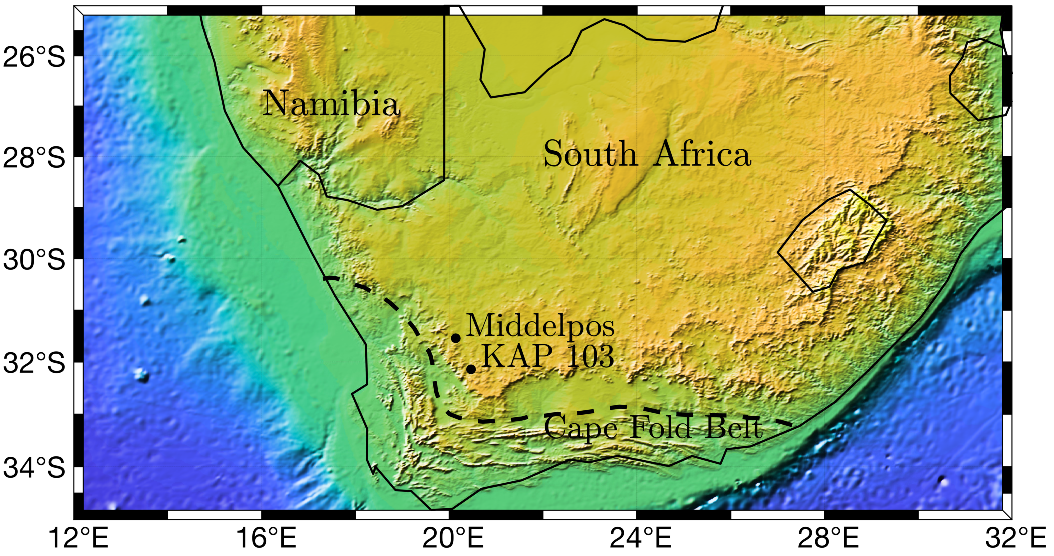
\includegraphics[width=\textwidth]{figures/map.pdf}
\caption{Location of Middelpos [$-31.544^\circ$, $20.141^\circ$] and KAP103 [$-32.139^\circ$, $20.468^\circ$] MT stations. Relief map is from \href{http://ngdc.noaa.gov/mgg/global/global.html}{the ETOPO1 Global Relief Model} and the Cape Fold Belt line was derived from digitization of Figure 1. of \href{https://agupubs.onlinelibrary.wiley.com/doi/pdf/10.1029/2000GL012587}{Nguuri et al., 2001}.}
\label{fig:map}
\end{figure}

\begin{figure}[h!]
\centering
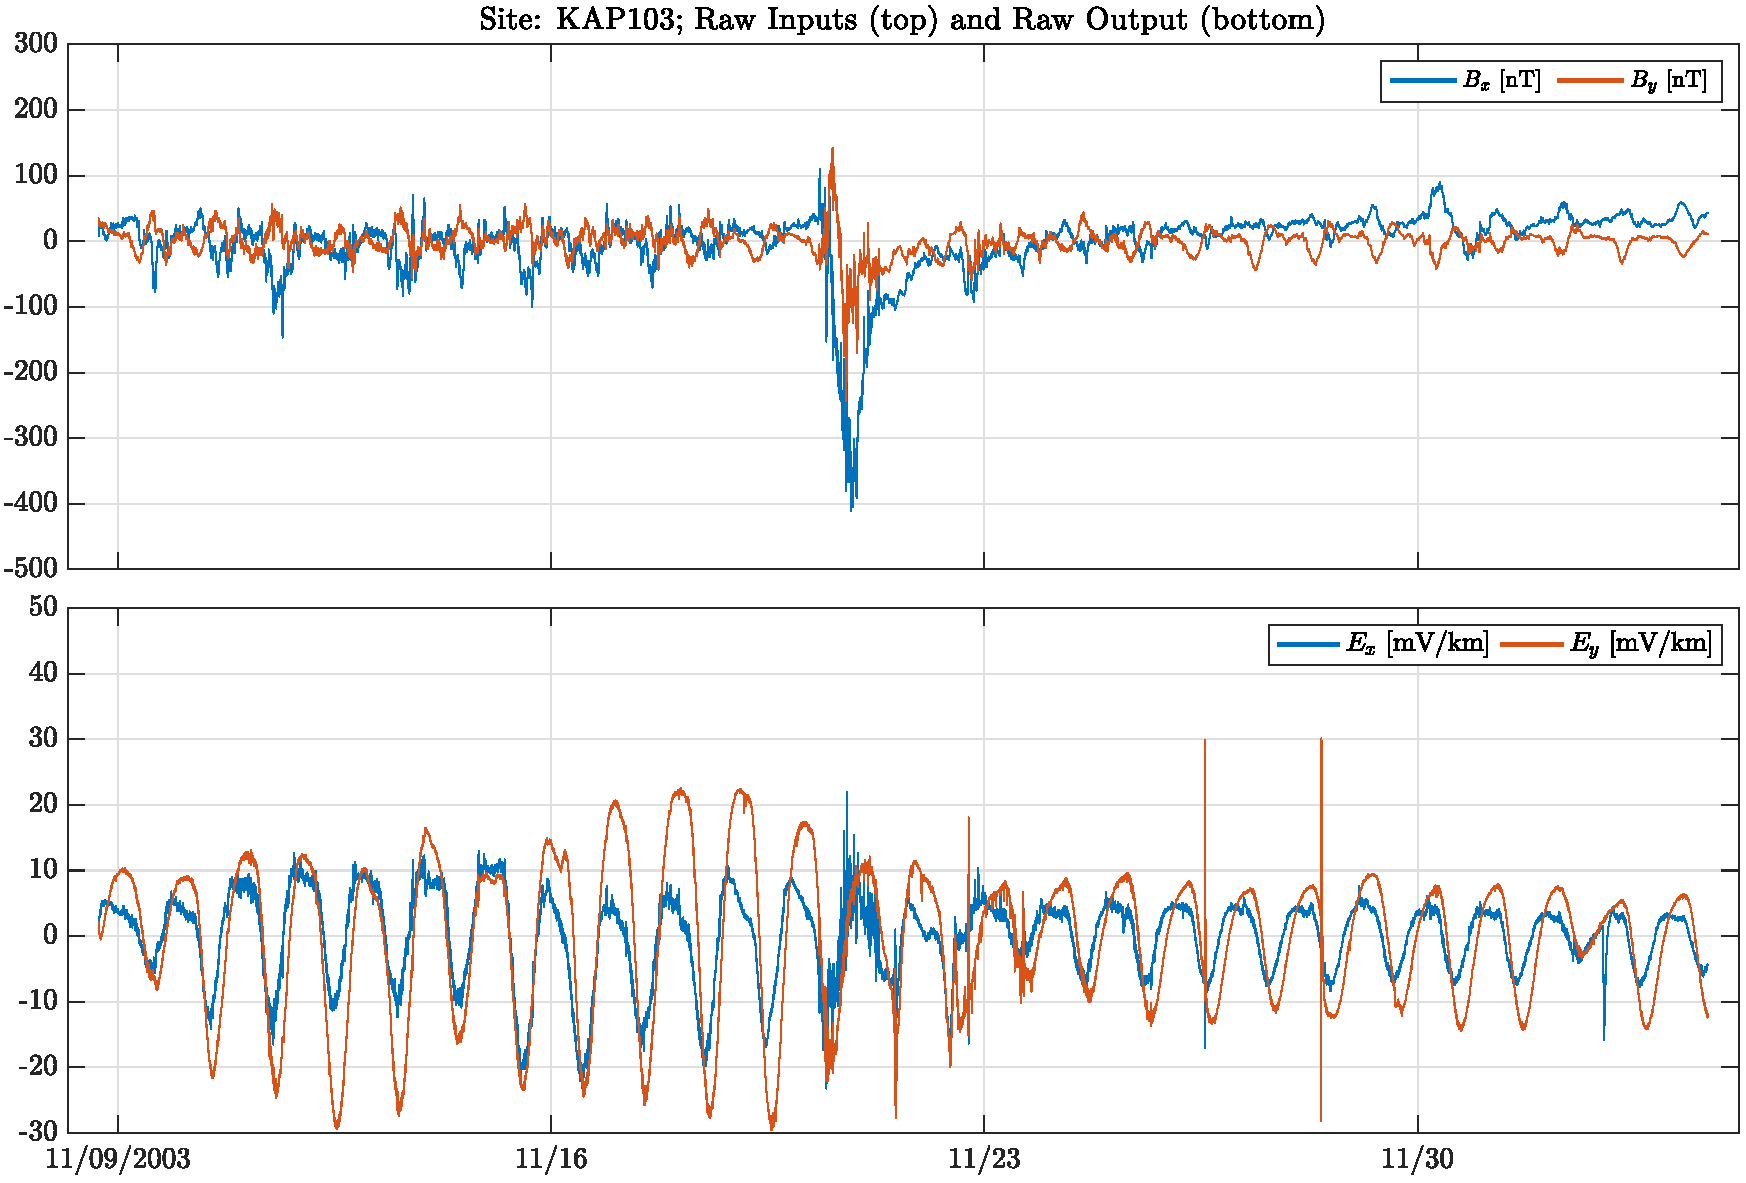
\includegraphics[width=\textwidth]{figures/KAP103/timeseries.pdf}
\caption{5-second-cadence measurements from the \href{https://www.mtnet.info/data/samtex/samtex.html}{MTNet SAMTEX page}; See also Jones et al. (2009).}
\label{fig:KAP103_timeseries}
\end{figure}

\clearpage

\section{Results - KAP103 TFs only}

Legend labels

\begin{itemize}

    \item OLS 26 1-day segments - Average of 26 1-day TF estimates. Transfer function estimates were made using the standard OLS method in the frequency domain using logarithmically spaced evaluation frequencies (indicated by dots in the following figures). Similar results were obtained using the (robust) transfer function estimate program provided with a LEMI instrument and our own implementation of robust regression with a hard cut-off bast on the MT literature.

    \item BIRRP - TF estimate derived using the Bounded Influence Remote Reference Program (Chave and Thomson, 2004), apparently derived using measurements at $\sim$10-second cadence. TFs were obtained from the \href{https://www.mtnet.info/data/samtex/samtex.html}{MTNet SAMTEX page}; See Jones et al. (2009) for documentation on the calculation.

\end{itemize}

\clearpage

\subsection{$E_x$ response}

\begin{figure}[h!]
\centering
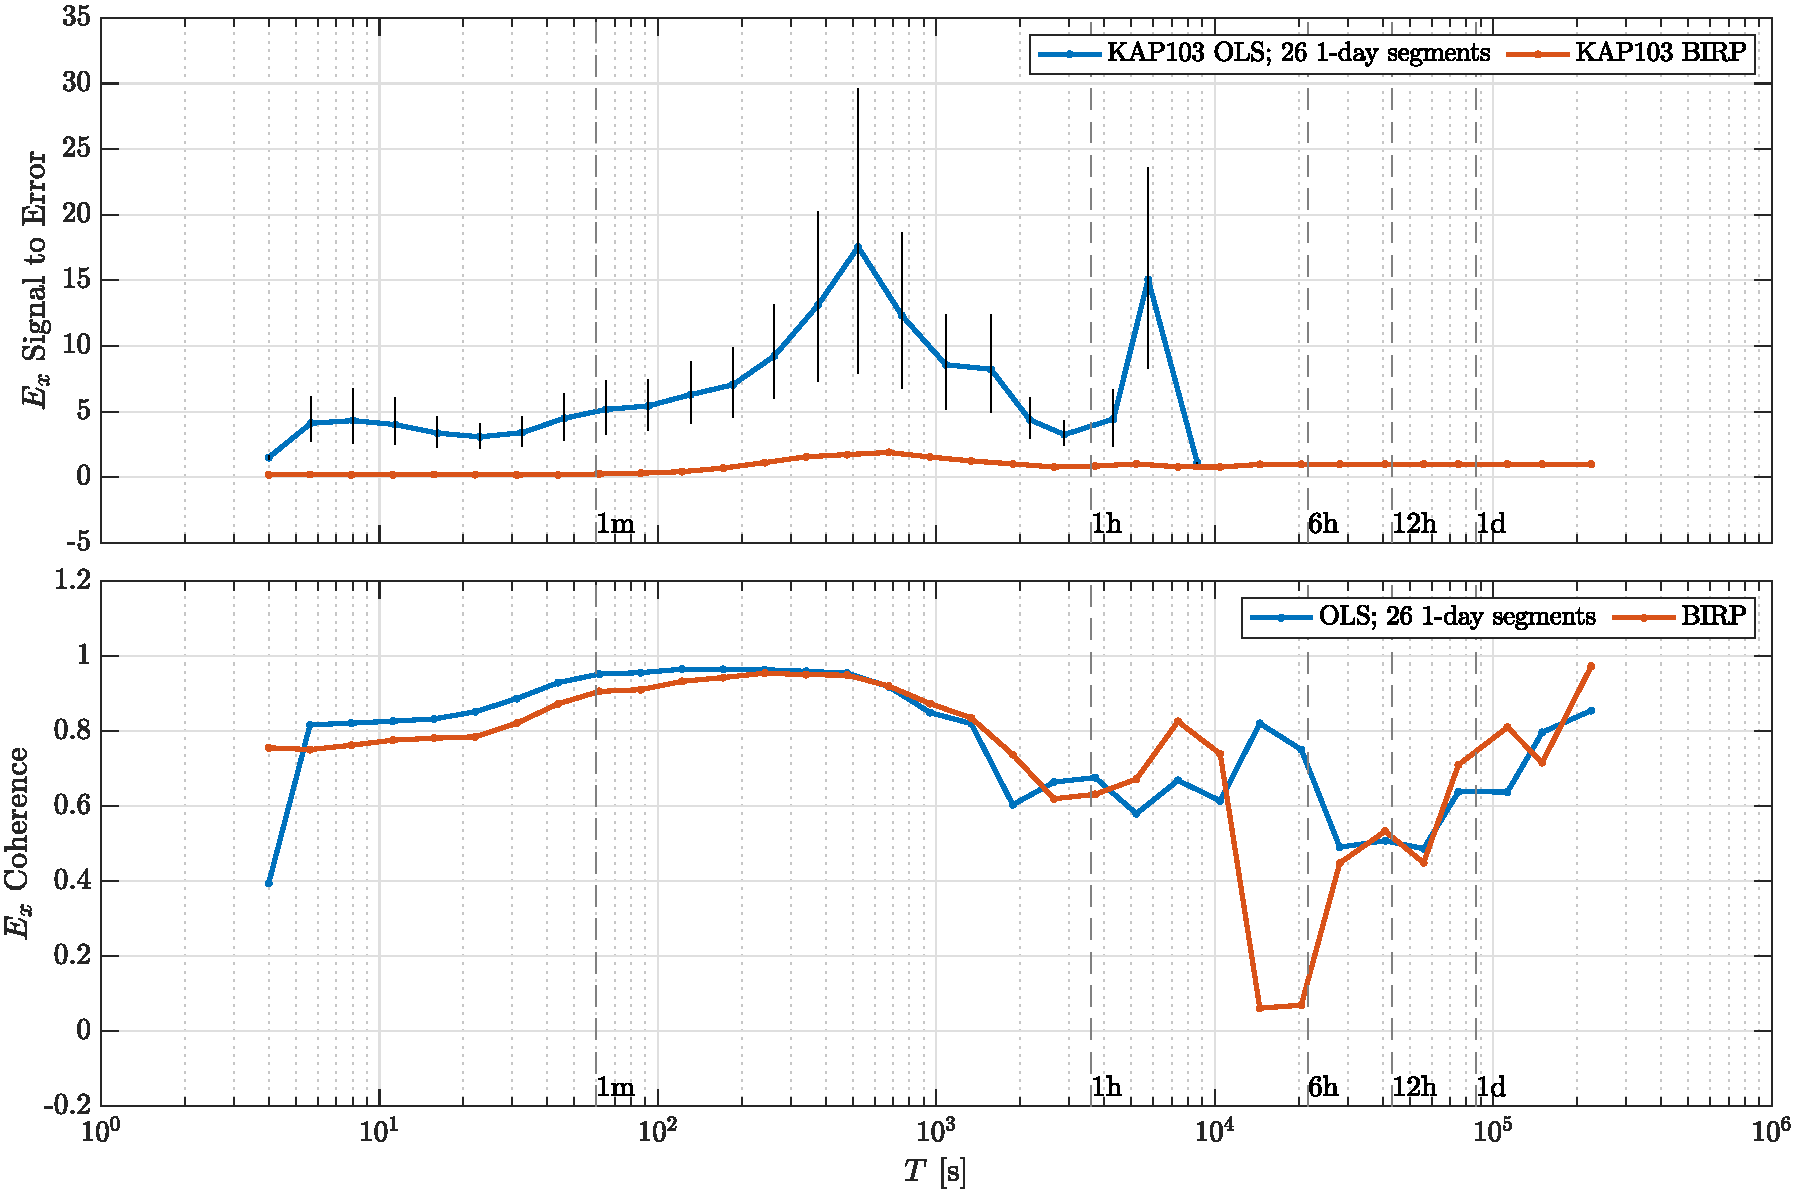
\includegraphics[width=\textwidth]{figures/KAP103/SN_compare-E_x.pdf}
\caption{(top) Signal to Error ratio versus period. The signal spectrum is the raw spectrum of the 5-second cadence $E_x$ averaged in bins centered on the evaluation frequencies used for the TF estimates (indicated by dots). The error spectrum is the raw spectrum of the difference between the 5-second cadence $E_x$ and that predicted using the TF; the error spectrum was averaged in the same way as the signal spectrum. The ratio of these averaged spectra at each evaluation frequency is shown. (bottom) Coherence averaged in bins centered on the evaluation frequencies used for the TF estimates. Note that these are in-sample measures of model performance.}
\label{fig:universe}
\end{figure}

\clearpage

\begin{figure}[h!]
\centering
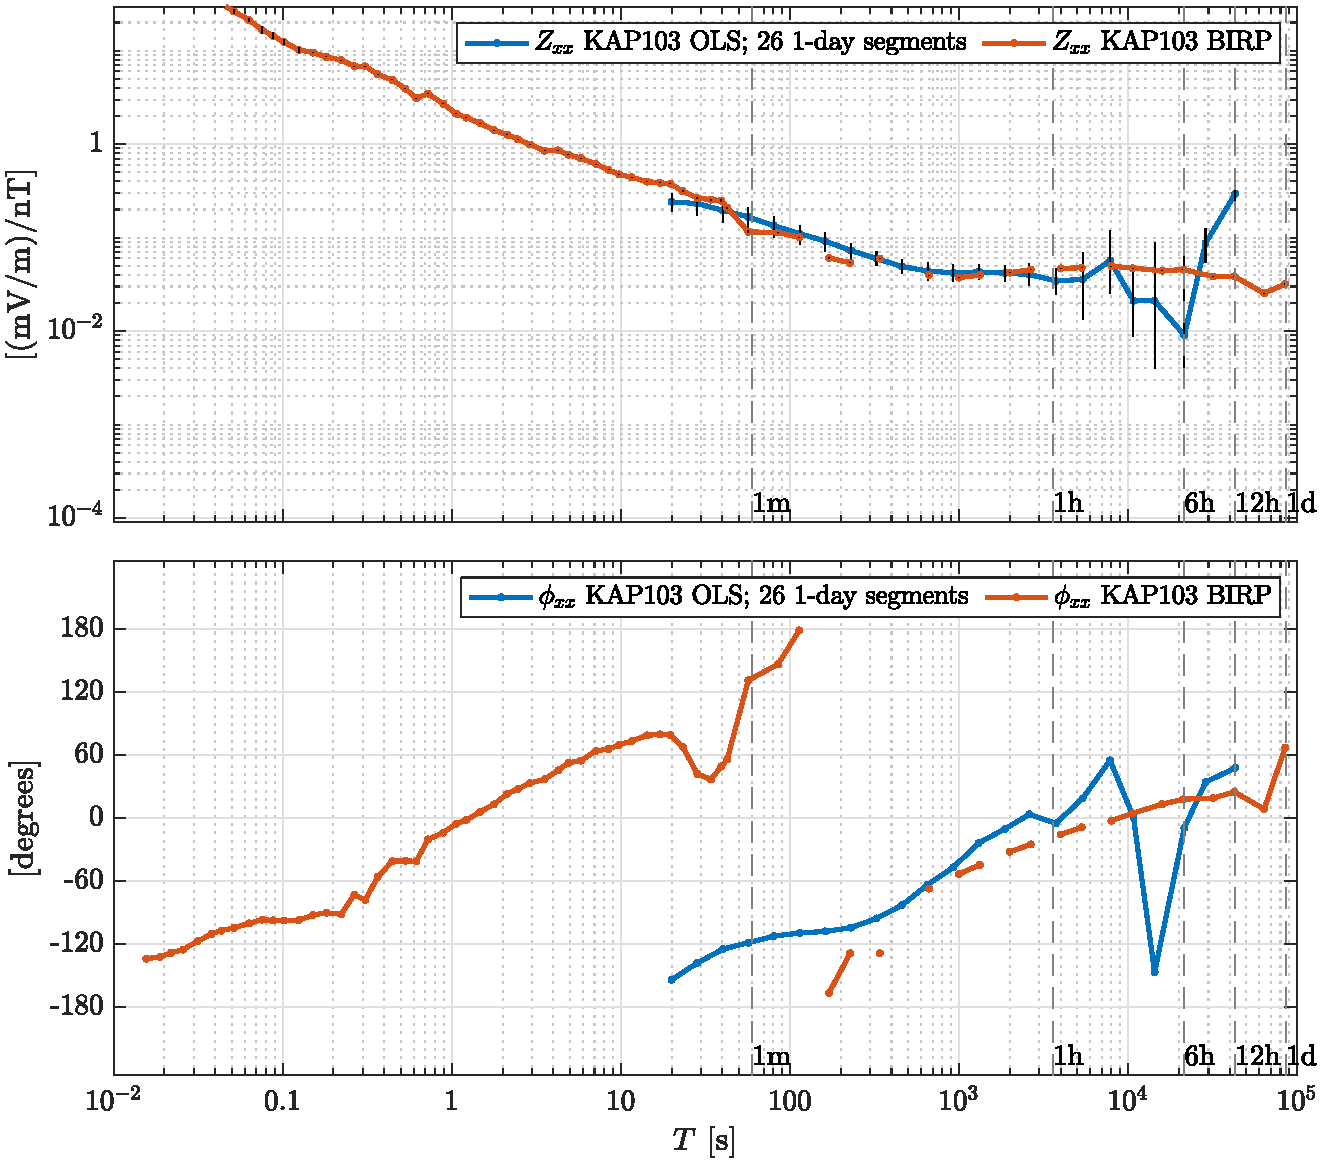
\includegraphics[width=\textwidth]{figures/KAP103/transferfnZ_compare-Z_xx_Magnitude_Phase.pdf}
\caption{}
\end{figure}

\clearpage

\begin{figure}[h!]
\centering
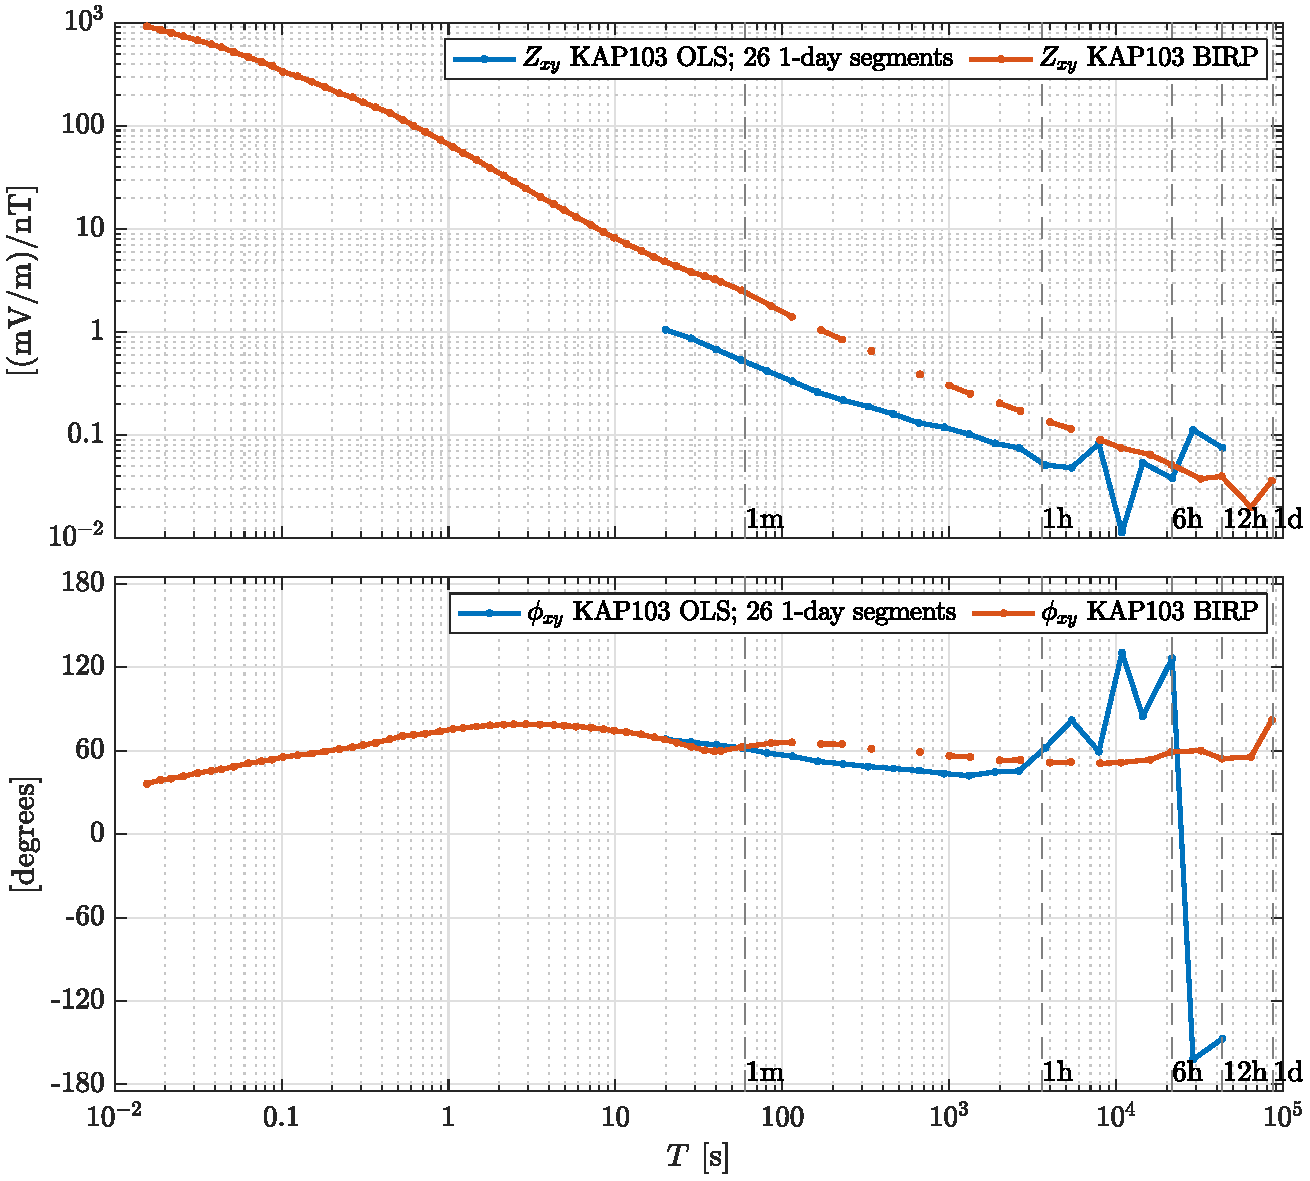
\includegraphics[width=\textwidth]{figures/KAP103/transferfnZ_compare-Z_xy_Magnitude_Phase.pdf}
\caption{}
\label{fig:universe}
\end{figure}

\clearpage

\subsection{$E_y$ response}

\begin{figure}[h!]
\centering
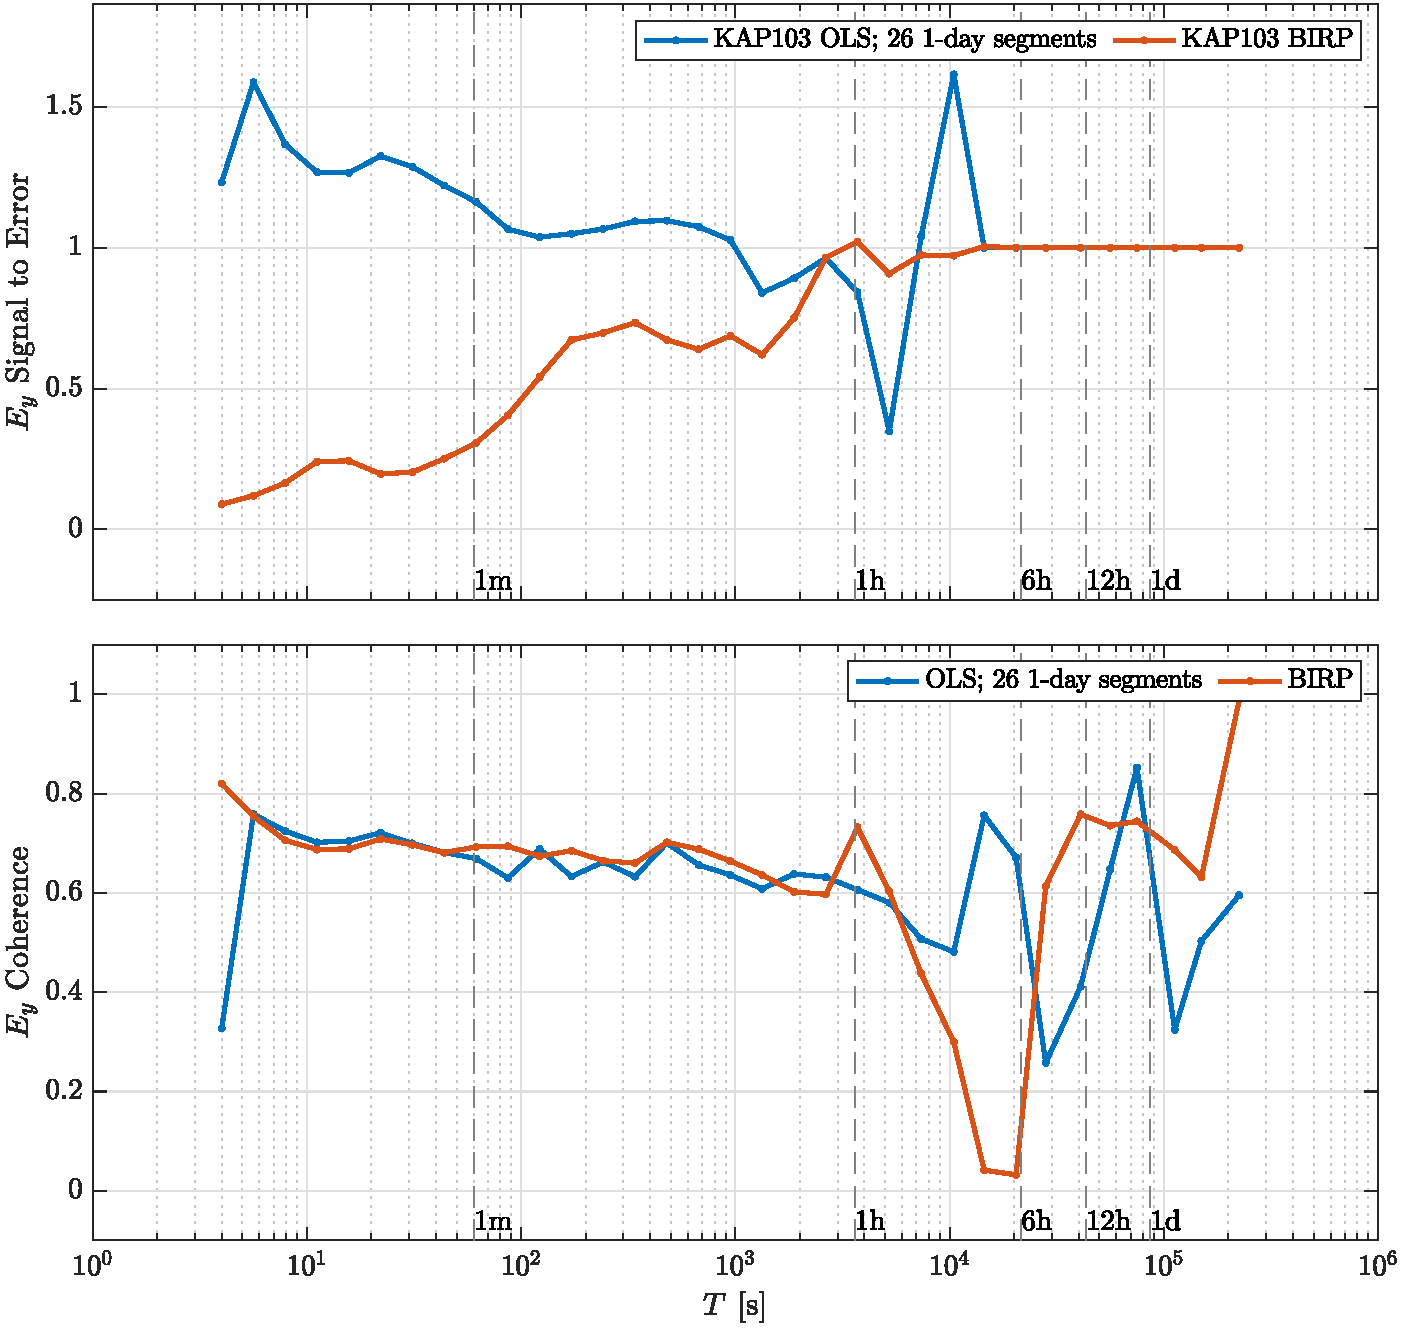
\includegraphics[width=\textwidth]{figures/KAP103/SN_compare-E_y.pdf}
\caption{Signal to Error and coherence for $E_y$.}
\label{fig:universe}
\end{figure}

\clearpage

\begin{figure}[h!]
\centering
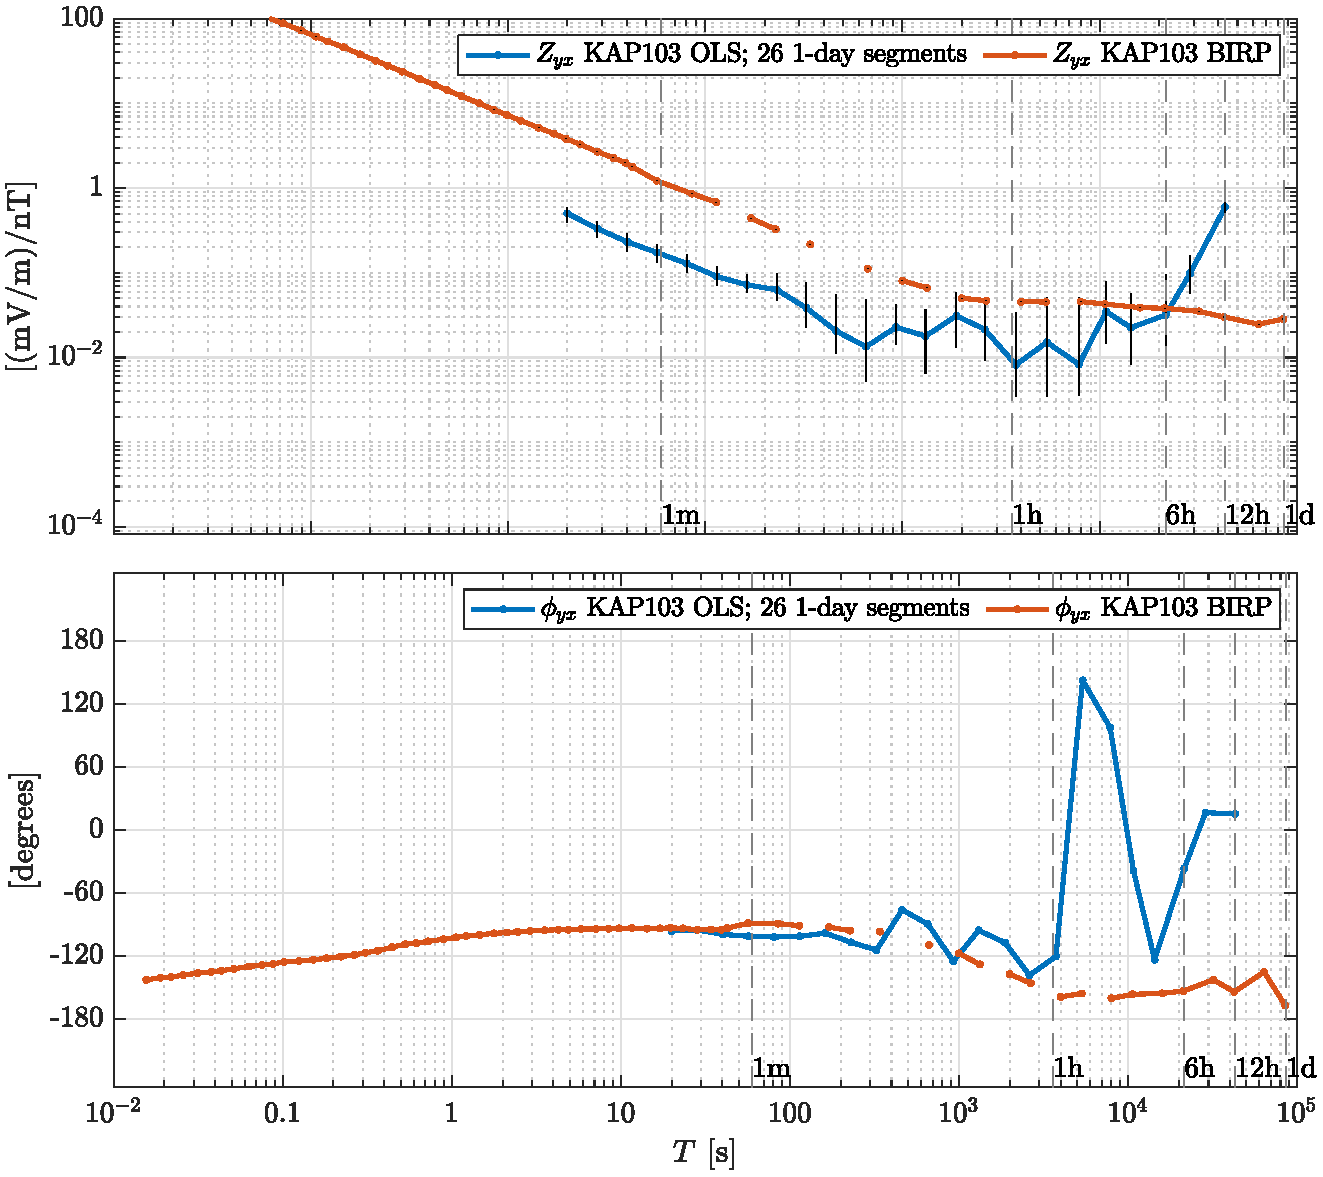
\includegraphics[width=\textwidth]{figures/KAP103/transferfnZ_compare-Z_yx_Magnitude_Phase.pdf}
\caption{}
\label{fig:universe}
\end{figure}

\begin{figure}[h!]
\centering
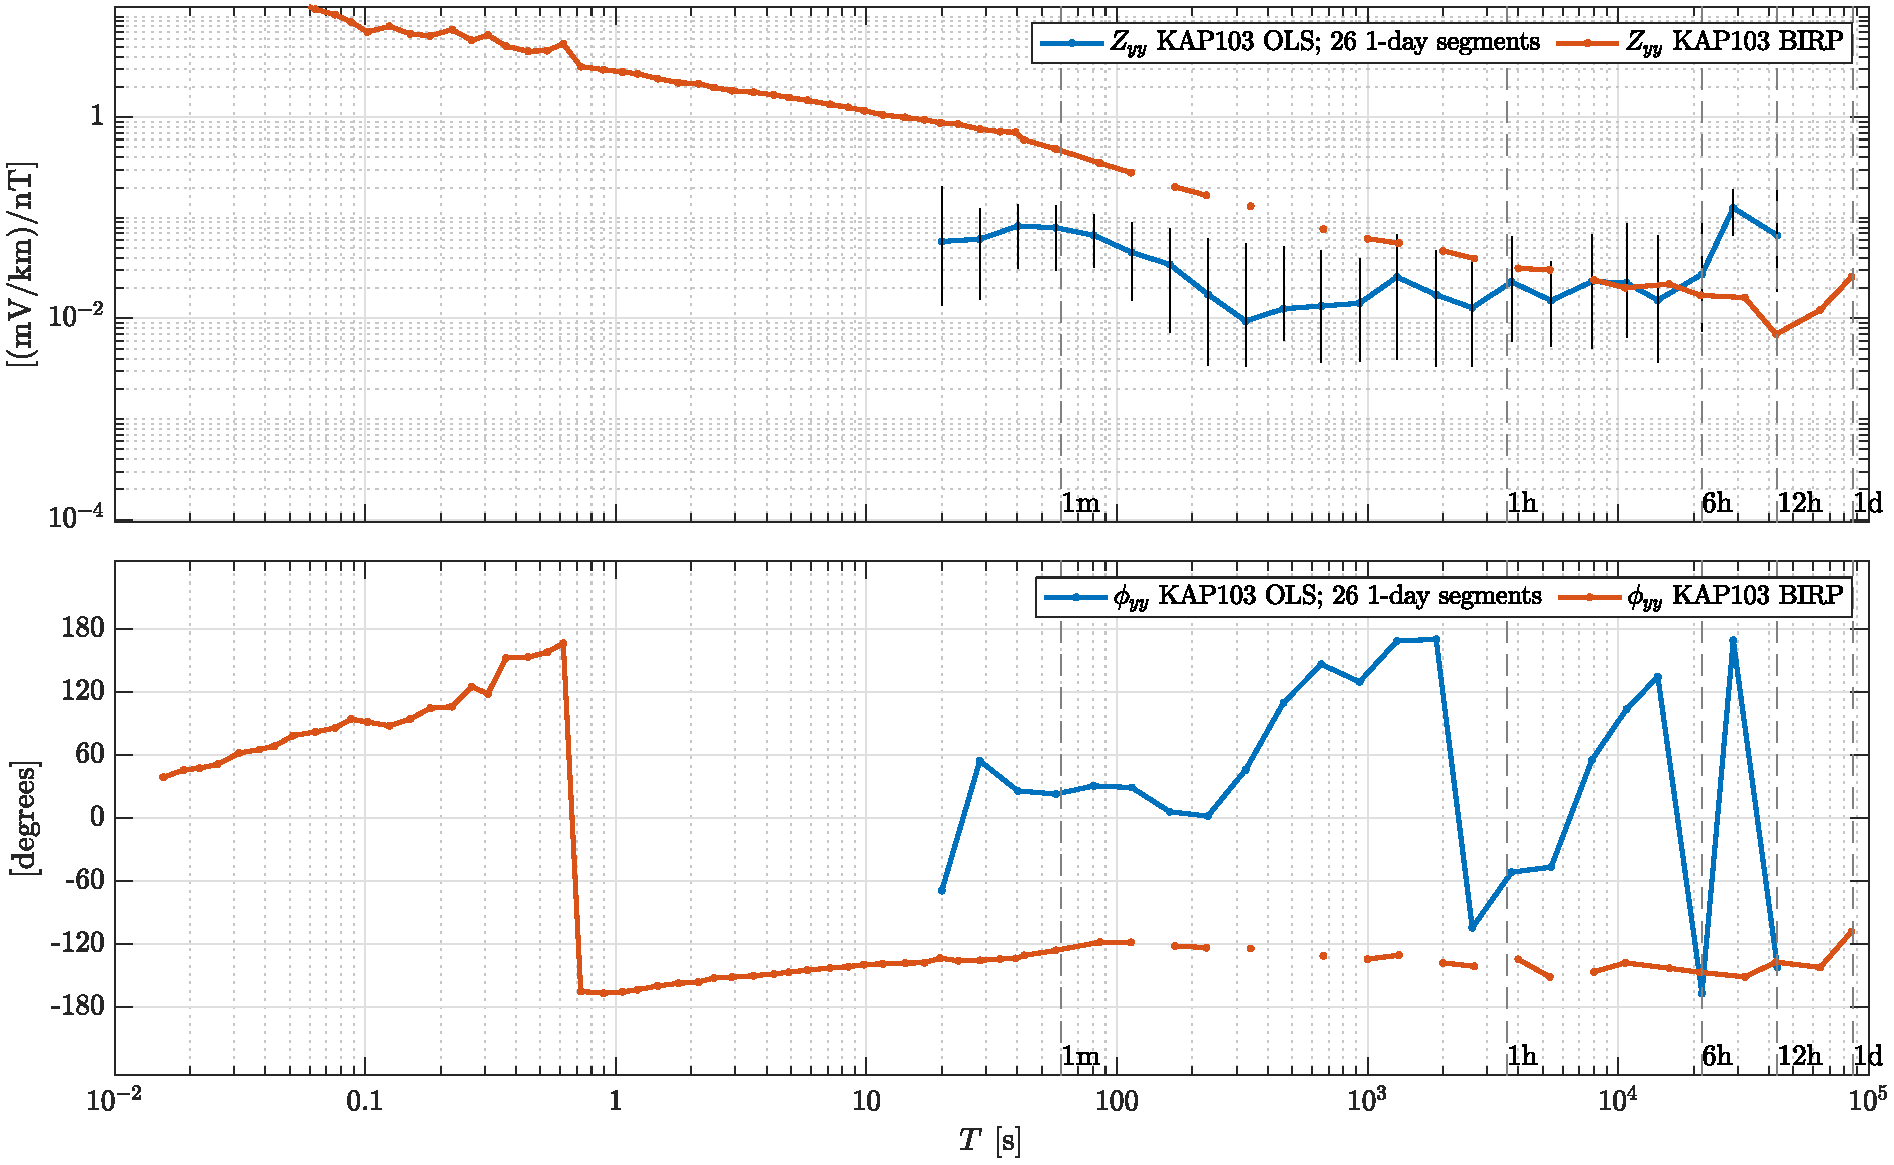
\includegraphics[width=\textwidth]{figures/KAP103/transferfnZ_compare-Z_yy_Magnitude_Phase.pdf}
\caption{}
\label{fig:universe}
\end{figure}

\clearpage

\section{Results KAP103 and Middelpos TFs}


\begin{itemize}

    \item OLS 55 1-day segments - 55 days of data are available from Middelpos. The method used is the same aas that for OLS 26 1-day for KAP103.

    \item OLS 26 1-day segments - Transfer function derived using 26 1-day segments from KAP103 in 2003. See previous section for calculation details.
    
    \item BIRRP - Transfer function derived using data from KAP103 in 2003 with the BIRRP algorithm. See previous section for calculation details.
    
\end{itemize}

\begin{figure}[h!]
\centering
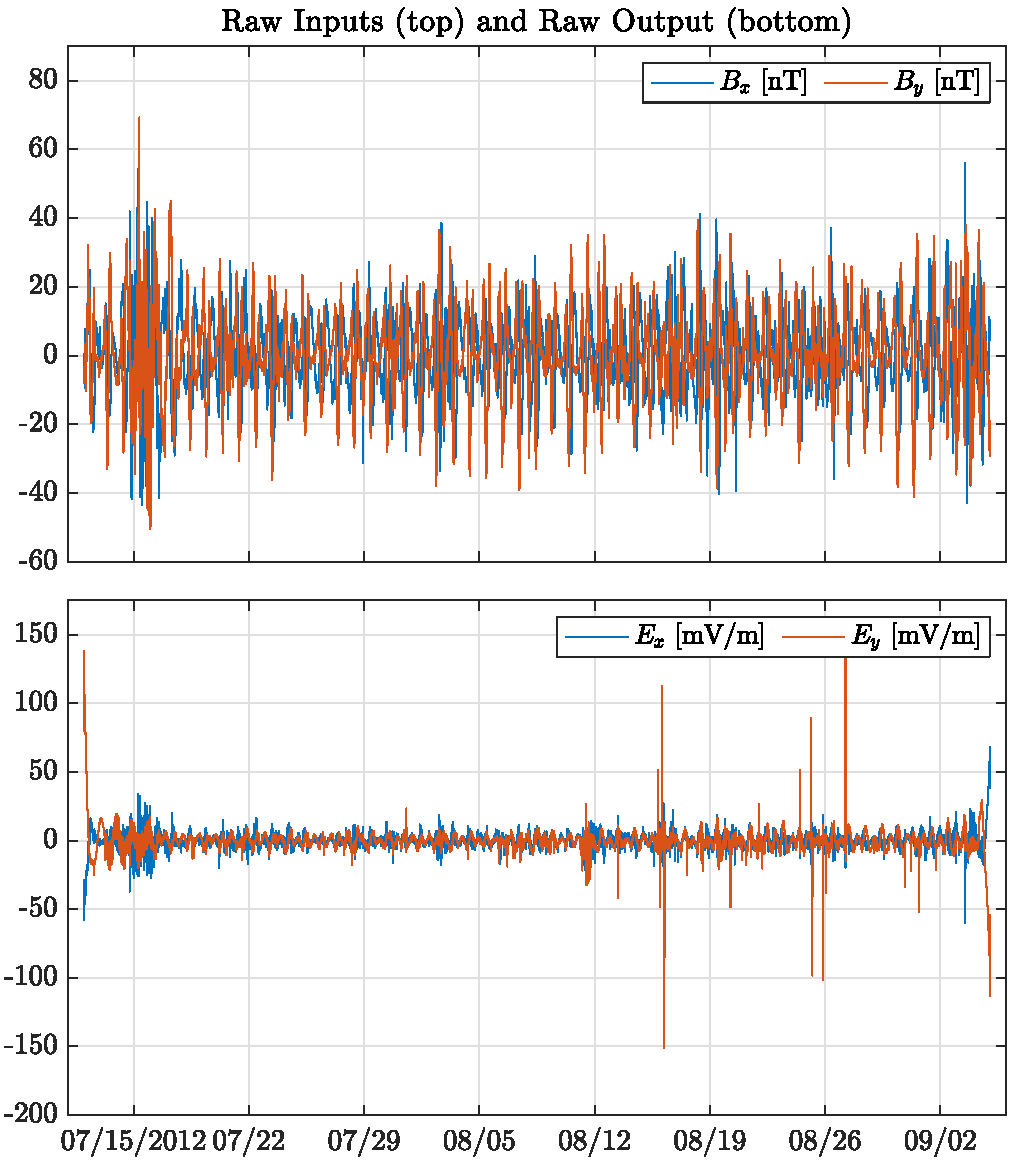
\includegraphics[width=\textwidth]{figures/Middelpos/timeseries.pdf}
\caption{1-second-cadence measurements from Middelpos.}
\label{fig:KAP103_timeseries}
\end{figure}

\clearpage


\begin{figure}[h!]
\centering
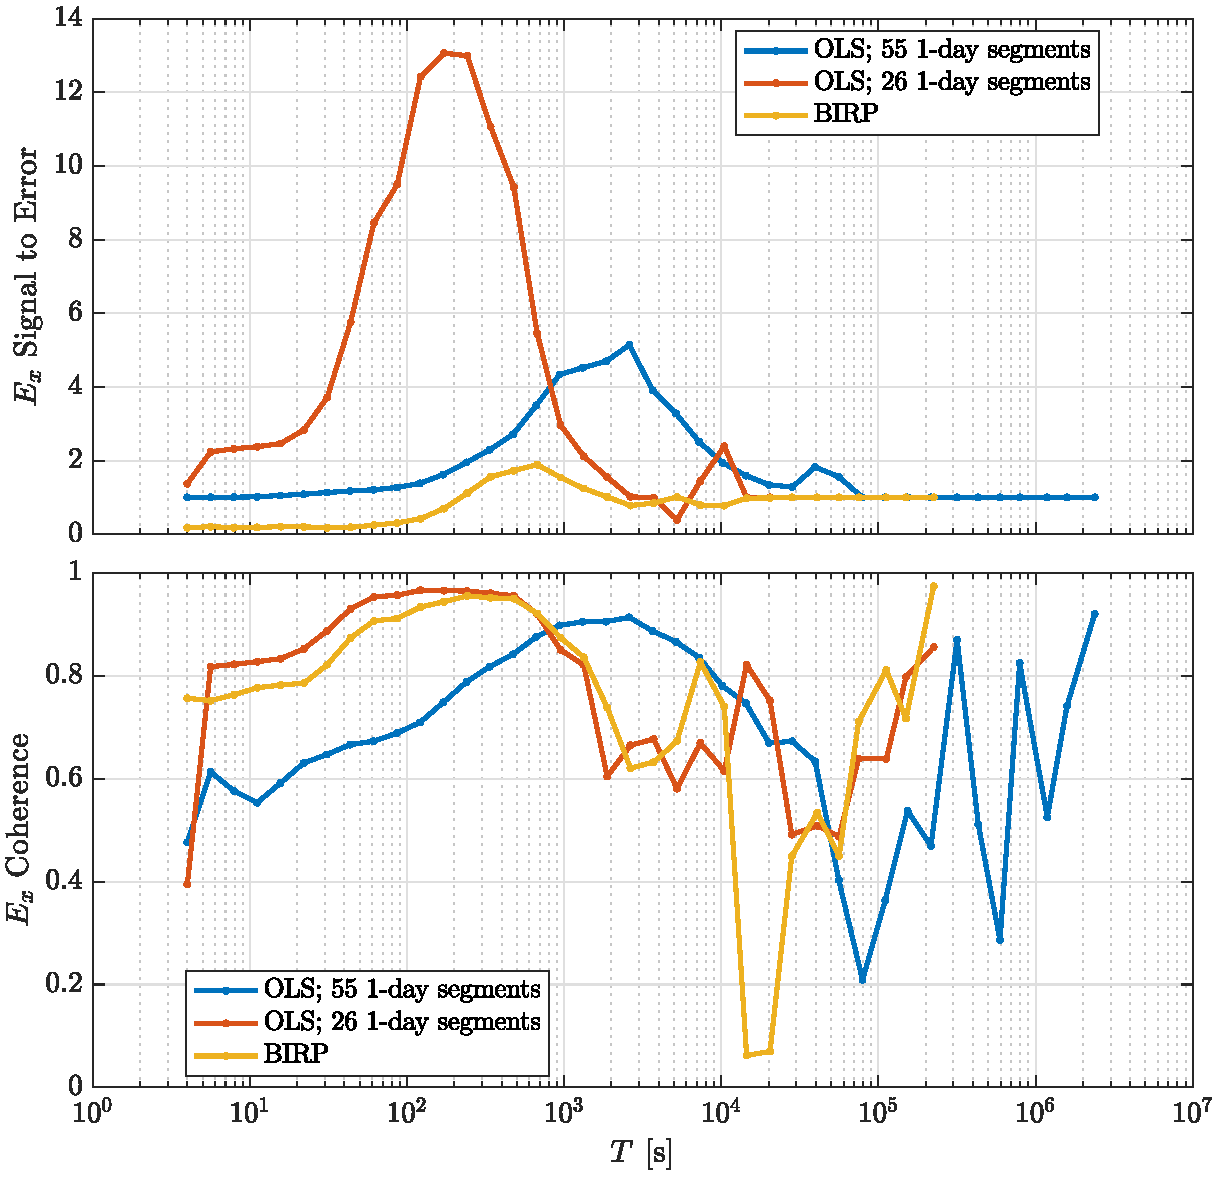
\includegraphics[width=\textwidth]{figures/KAP103_Middelpos/SN_compare-E_x.pdf}
\caption{(top) Signal to Error ratio versus period. The signal spectrum is the raw spectrum of the 5-second cadence $E_x$ averaged in bins centered on the evaluation frequencies used for the TF estimates (indicated by dots). The error spectrum is the raw spectrum of the difference between the 5-second cadence $E_x$ and that predicted using the TF; the error spectrum was averaged in the same way as the signal spectrum. The ratio of these averaged spectra at each evaluation frequency is shown. (bottom) Coherence averaged in bins centered on the evaluation frequencies used for the TF estimates. Note that these are in-sample measures of model performance.}
\label{fig:universe}
\end{figure}

\clearpage

\begin{figure}[h!]
\centering
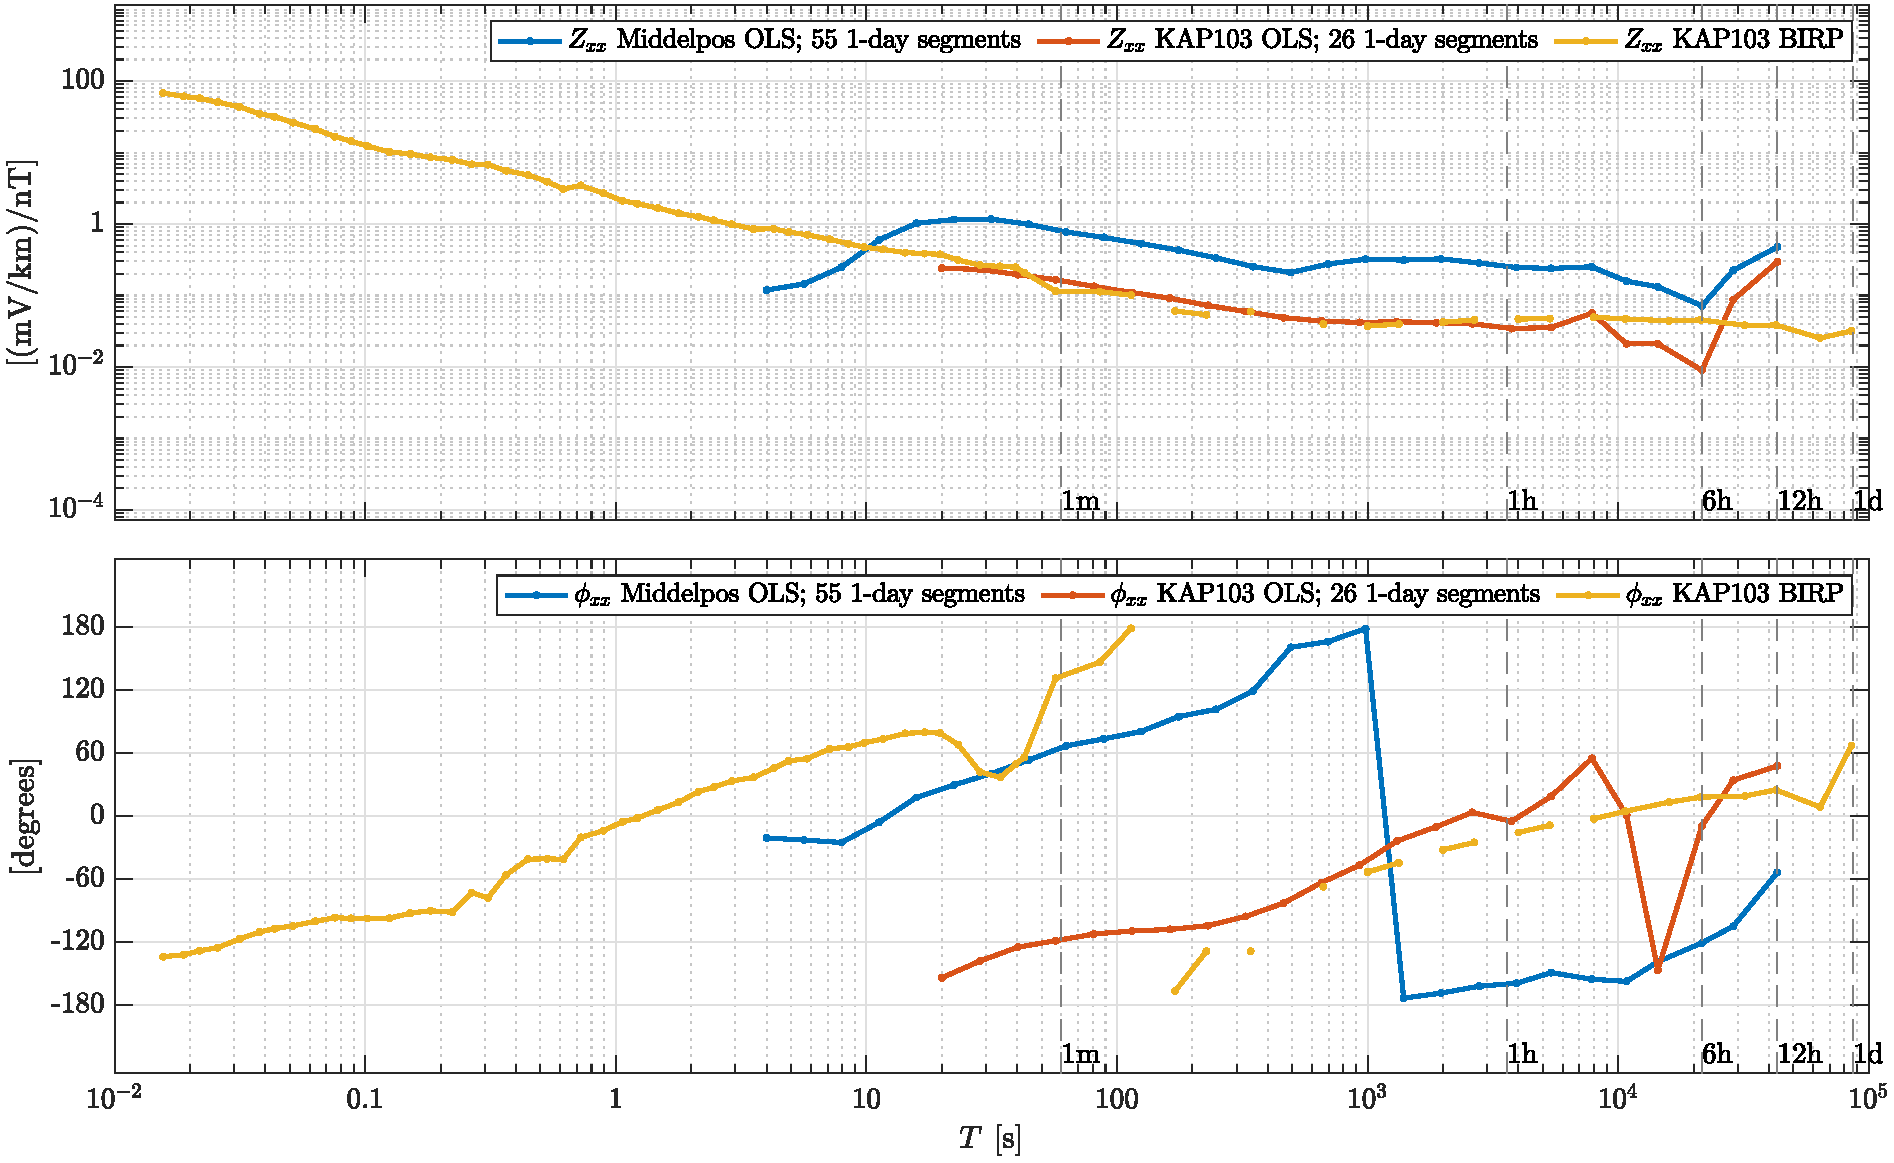
\includegraphics[width=\textwidth]{figures/KAP103_Middelpos/transferfnZ_compare-Z_xx_Magnitude_Phase.pdf}
\caption{}
\end{figure}

\clearpage

\begin{figure}[h!]
\centering
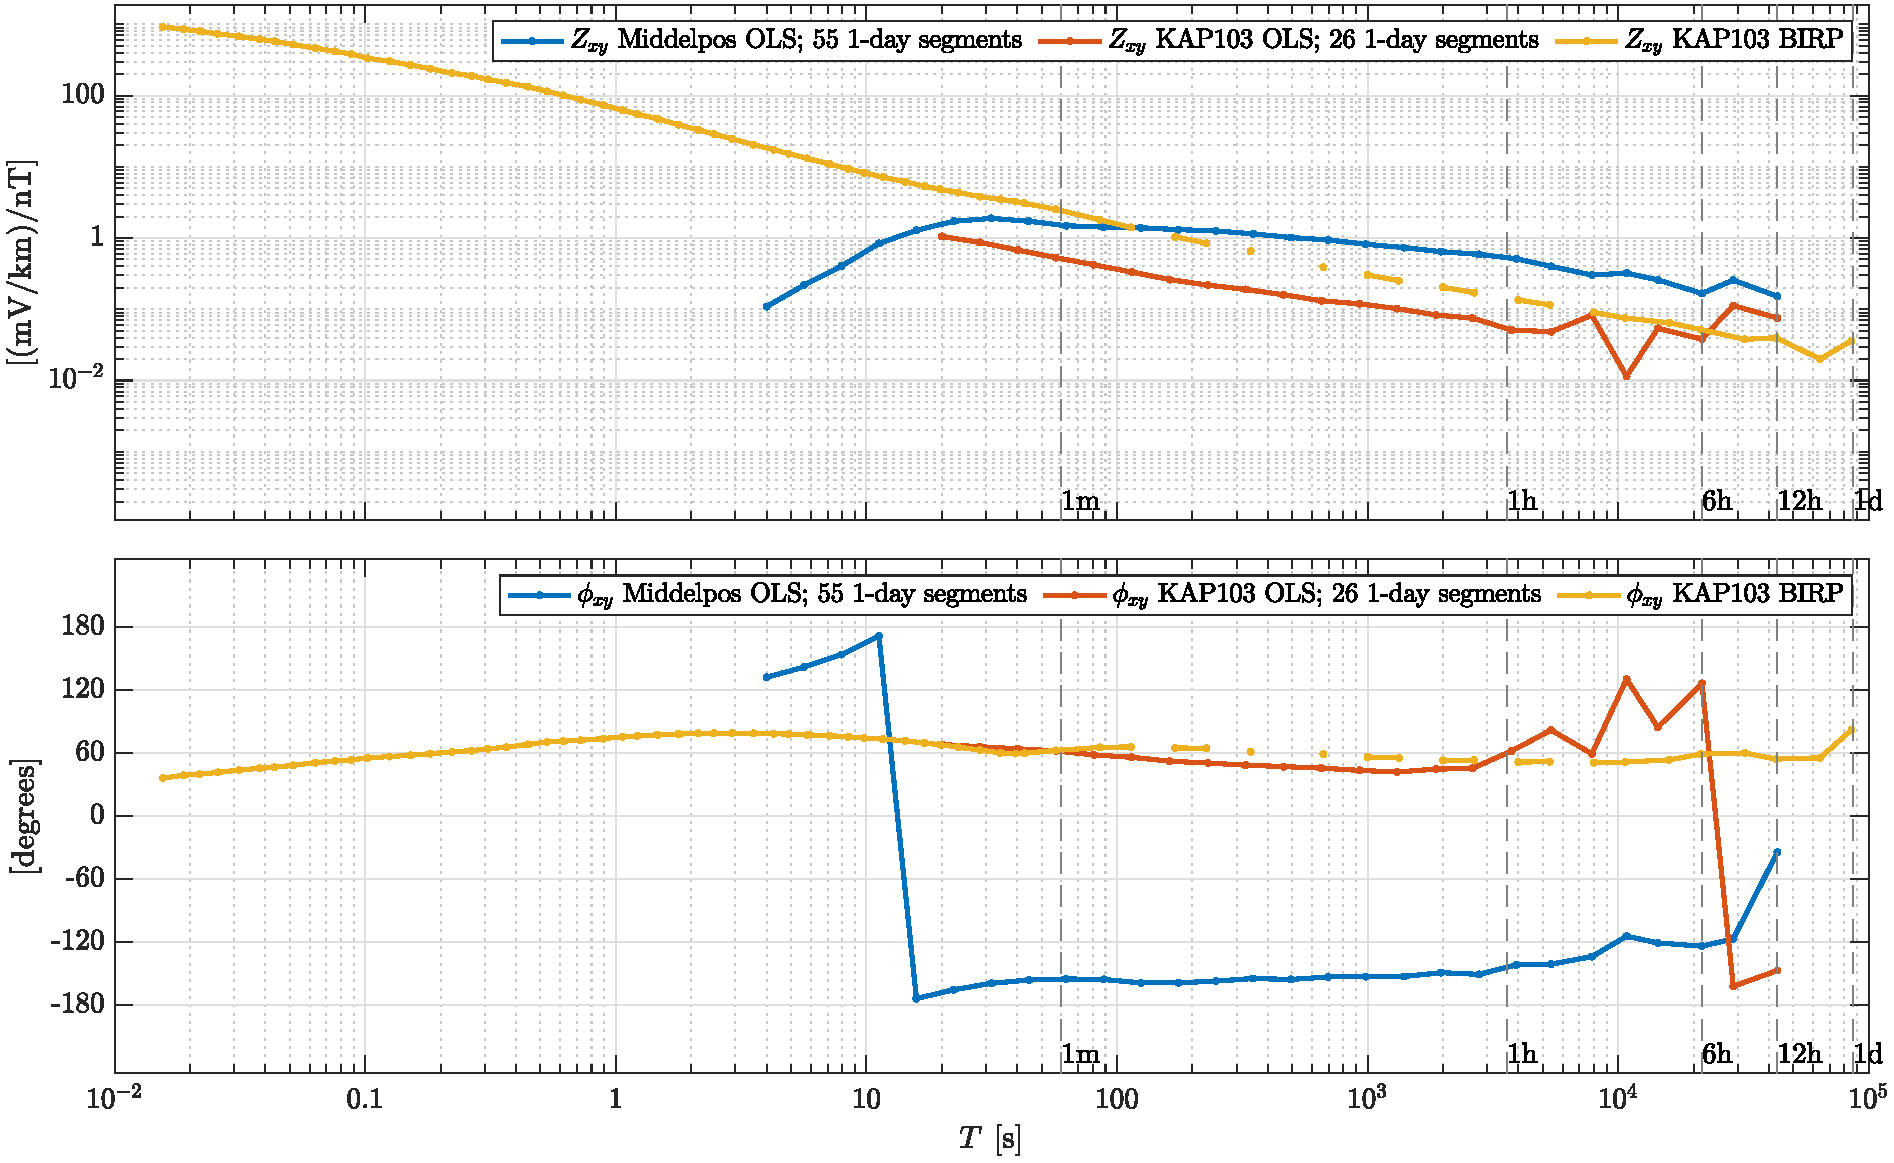
\includegraphics[width=\textwidth]{figures/KAP103_Middelpos/transferfnZ_compare-Z_xy_Magnitude_Phase.pdf}
\caption{}
\label{fig:universe}
\end{figure}

\clearpage

\subsection{$E_y$ response}

\begin{figure}[h!]
\centering
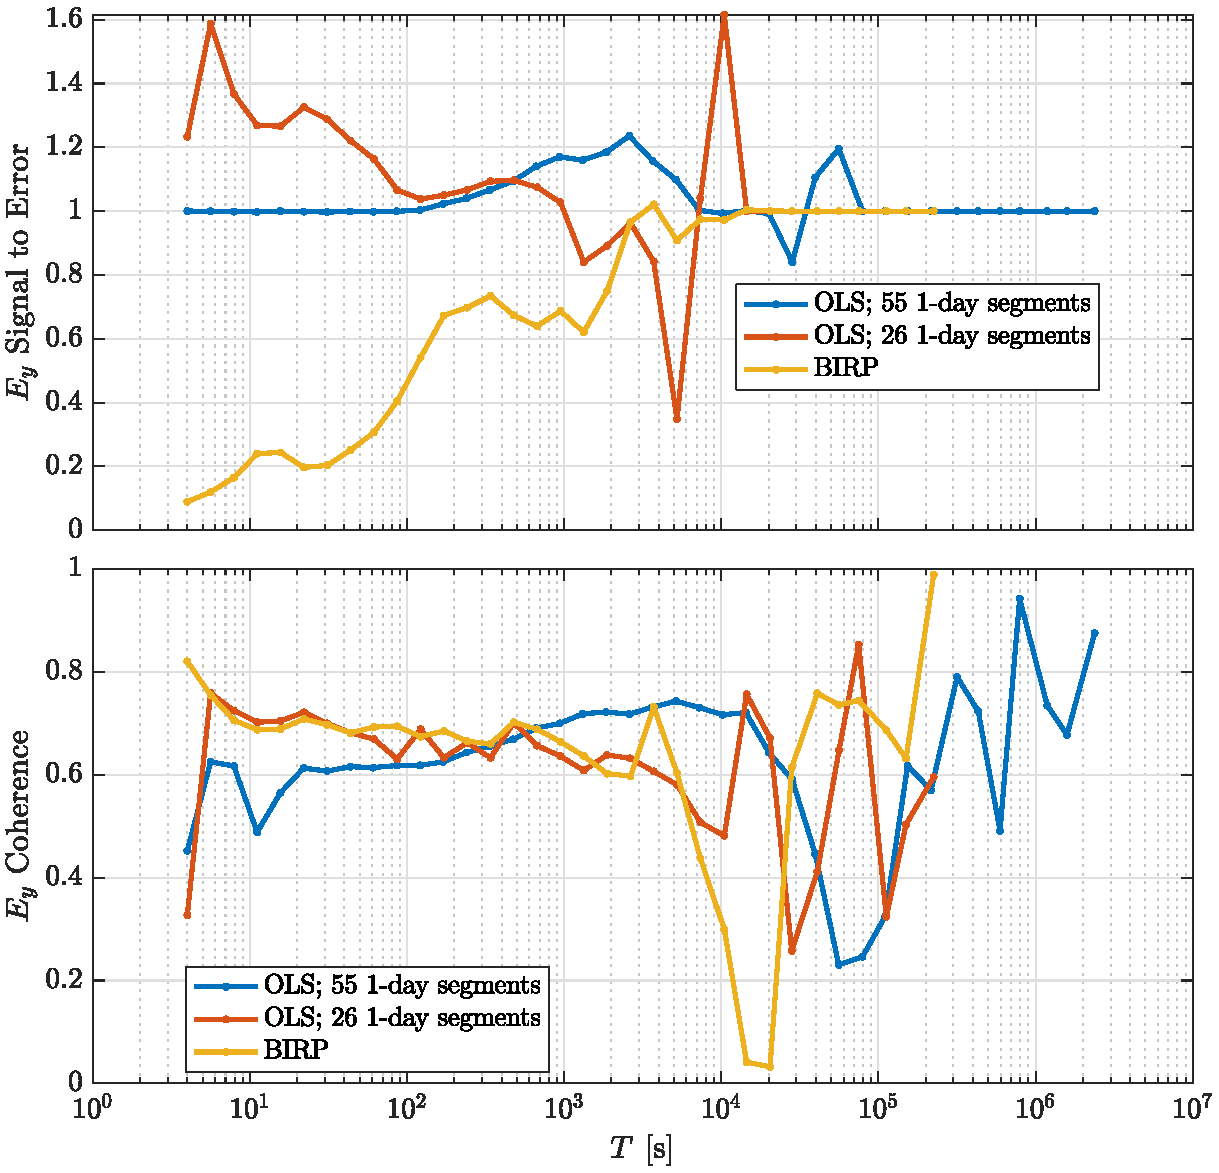
\includegraphics[width=\textwidth]{figures/KAP103_Middelpos/SN_compare-E_y.pdf}
\caption{Signal to Error and coherence for $E_y$.}
\label{fig:universe}
\end{figure}

\clearpage

\begin{figure}[h!]
\centering
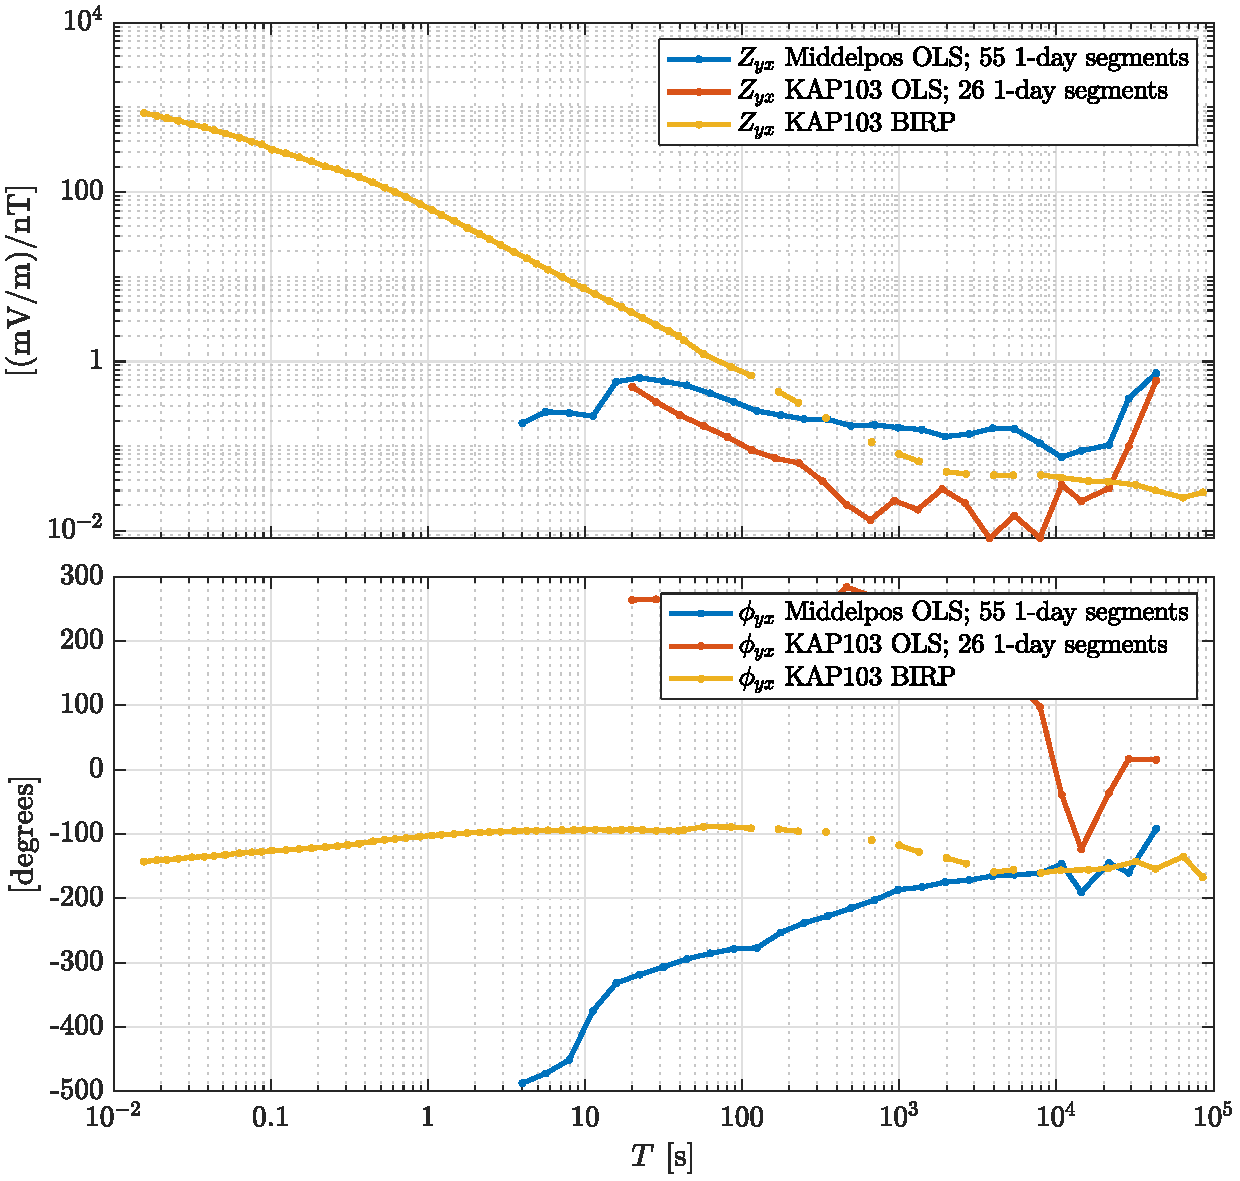
\includegraphics[width=\textwidth]{figures/KAP103_Middelpos/transferfnZ_compare-Z_yx_Magnitude_Phase.pdf}
\caption{}
\label{fig:universe}
\end{figure}

\begin{figure}[h!]
\centering
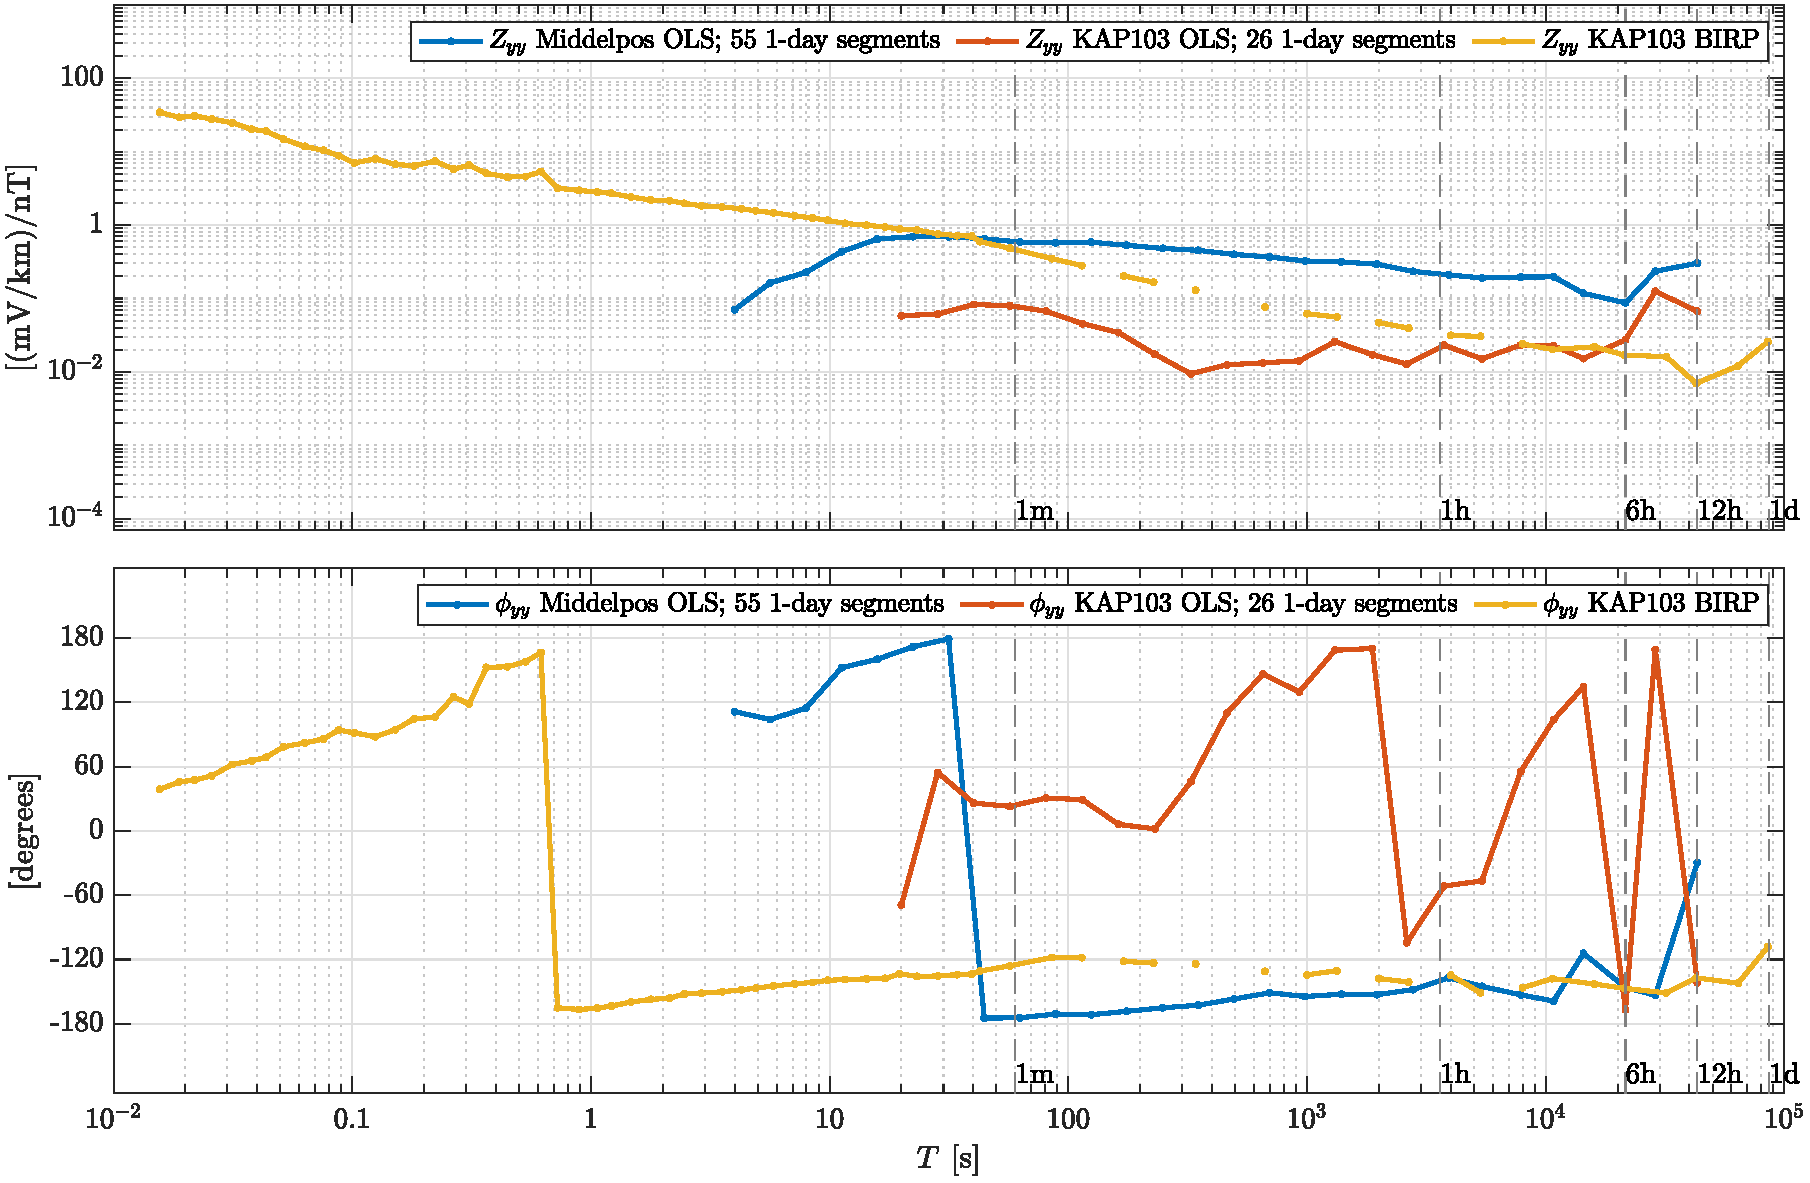
\includegraphics[width=\textwidth]{figures/KAP103_Middelpos/transferfnZ_compare-Z_yy_Magnitude_Phase.pdf}
\caption{}
\label{fig:universe}
\end{figure}

\clearpage


\end{document}
